\documentclass{beamer}
\usepackage{subcaption}
\usepackage{float}
\usepackage{setspace}
\usepackage{wrapfig}
\usepackage{caption}
\captionsetup[figure]{labelformat=empty}
\usetheme[pageofpages=of,% String used between the current page and the
                         % total page count.
          bullet=circle,% Use circles instead of squares for bullets.
          titleline=true,% Show a line below the frame title.
          alternativetitlepage=true,% Use the fancy title page.
          titlepagelogo=logo-polito,% Logo for the first page.
          watermark=watermark-polito,% Watermark used in every page.
          watermarkheight=100px,% Height of the watermark.
          watermarkheightmult=4,% The watermark image is 4 times bigger
                                % than watermarkheight.
          ]{Theme}
\usepackage{lmodern}
\author{\small By\\Bharat Bhushan (153100048)}
\title{{{Thermoelastic fracture problems using Extended Finite Element Method}}}
\institute{\small Under the guidance of\\Prof. Salil S. Kulkarni\\ \vspace{5pt}Department of Mechanical Engineering, IIT Bombay}
\date{\vspace{-5pt}October 18, 2016}
\begin{document}
%%%%%%%%%%%%%%%%%%%%%%%%%%%%%%%%%%%%%%%%%%%%%%%%%%%%%%%%%%%%%%%%%%%%5
%%%% TITLE PAGE %%%%%%%%%%%%%%%%%%%%%%%%%%%%%%%%%%%%%%%%%%%%%%%%%%%%
%%%%%%%%%%%%%%%%%%%%%%%%%%%%%%%%%%%%%%%%%%%%%%%%%%%%%%%%%%%%%%%%%%%%%
\begin{frame}[t,plain]
\titlepage
\end{frame}
%%%%%%%%%%%%%%%%%%%%%%%%%%%%%%%%%%%%%%%%%%%%%%%%%%%%%%%%%%%%%%%%%%%%%%
%%%% content %%%%%%%%%%%%%%%%%%%%%%%%%%%%%%%%%%%%%%%%%%%%%%%%%%%%%%%
%%%%%%%%%%%%%%%%%%%%%%%%%%%%%%%%%%%%%%%%%%%%%%%%%%%%%%%%%%%%%%%%%%%%

%%%%%%%%%%%%%%%%%%%%%%%%%%%%%%%%%%%%%%%%%%%%%%%%%%%%%%%%%%%%%%%%%
\begin{frame}[t,fragile]{Outline}
    \begin{itemize}
        \item Introduction  
        \item Motivation 
        \item Literature Survey 
        \item Work done 
        \item Problem definition 
        \item Conclusion 
    \end{itemize}
\end{frame}
%%%%%%%%%%%%%%%%%%%%%%%%%%%%%%%%%%%%%%%%%%%%%%%%%%%%%%%%%%%%%%%%%
\begin{frame}[t,fragile]{Introduction: Thermo-elastic Fracture Problems}
    \vspace{-.3cm}
    \begin{itemize}
        \item Due to heat transfer, temperature field is set up in the material which induces thermal stresses in the body.
\item These stresses becomes large in the vicinity of a discontinuity i.e. crack tip. If temperature variation is sufficiently large, it can lead to failure.
        \item Applications: Nuclear power plants, cylinder-nozzle
 intersection in pressure vessels, aerodynamic heating of high-speed aircraft, ultra fast pulse lasers etc.
   \end{itemize}
   \vspace{-.5cm}
\begin{figure}[H]
    \hspace{.7cm}
      \begin{subfigure}{0.45\textwidth}
    \centering
 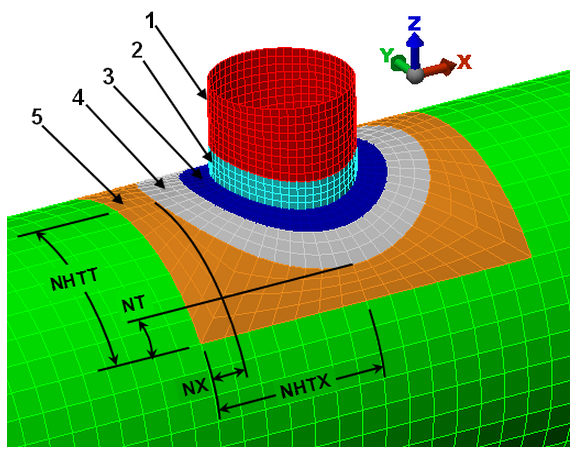
\includegraphics[scale=.1]{cyl.png}
 \caption{\tiny{The cylinder-nozzle intersection. (www.knowledge.autodesk.com)}}
 \label{cyl}
 \end{subfigure}
\begin{subfigure}{0.45\textwidth}
    \centering
 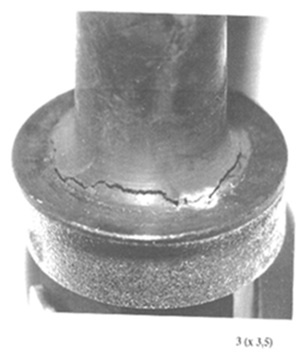
\includegraphics[scale=.1]{fail.jpg}
 \caption{\tiny{Cracked head of baffle bolt of Belgian Nuclear Reactor.(www.miningawareness.wordpress.com)}}
 \label{fail}
 \end{subfigure}
 \end{figure}
 \vspace{-.3cm}
   \tiny
   \hspace{15pt}
   \textbf{source}: Tian, X., Shen. (2006). A direct finite element method study of generalized thermoelastic problems. \\
   \vspace{-7pt}
   \hspace{15pt}
   \emph{International Journal of Solids and Structures}, 43(7), 2050-2063.
\end{frame}
%%%%%%%%%%%%%%%%%%%%%%%%%%%%%%%%%%%%%%%%%%%%%%%%%%%%%%%%%%%%%%%%%o 
\begin{frame}[t,fragile]{Why thermal load on crack is important?}
    \vspace{-.3cm}
    \footnotesize
\begin{itemize}
    \item Atkinson has solved the Dirichlet problem for Laplace's equation on a pie shaped region as $u(x,y)= r^{\frac{\pi}{\phi}}\sin\alpha\theta,\  r>0,\ 0<\theta<\phi$
        \begin{itemize}
                \footnotesize
    \item If $0<\phi<\pi$:
        The first partial derivative of u with respect to x and y remains continuous as we approach towards the origin. 
    \item If $\pi<\phi<2\pi$:
        The first derivative u with respect to x and y are not continuous as (x,y) approaches the origin. 
    \end{itemize}
    \item When $\phi=2\pi$, the problem becomes a crack problem and displacement and derivative of displacement vary as $u \propto r^{\frac{1}{2}}$ and $u'\propto  r^{-\frac{1}{2}}$ respectively. 
    \item As thermo-elastic problems are also governed by Laplace's equation, temperature will vary as $r^{\frac{1}{2}}$ and heat fluxes will be unbounded at the crack tip. 
\end{itemize}
  \tiny
  \vspace{10pt}
  \hspace{10pt}
   \textbf{source}: Atkinson, K. E. (1997).
    \emph{The numerical solution of \\
  \hspace{10pt}
    integral equations of the second kind} (Vol. 4). \\
  \hspace{10pt}
    Cambridge university press.
\begin{wrapfigure}{r}{0.4\textwidth}
    \centering
    \vspace{-50pt}
    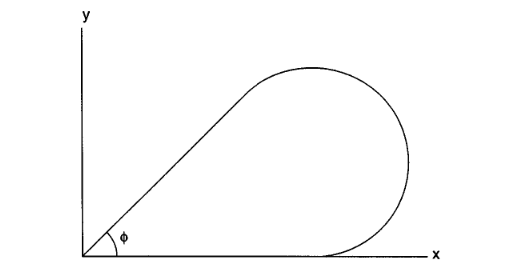
\includegraphics[width=.3\textwidth]{pie.png}
    \caption{\footnotesize Pie-shaped region.}
    \label{pie}
\end{wrapfigure}
 
\end{frame}
%%%%%%%%%%%%%%%%%%%%%%%%%%%%%%%%%%%%%%%%%%%%%%%%%%%%%%%%%%%%%%%%%%%%
\begin{frame}[t,fragile]{Methods of Solution}
    \vspace{-.4cm}
    \begin{itemize}
        \item Our main concern in case of thermally loaded fracture problems is to find the stress intensity factors. Methods for calculating stress intensity factors in FEM can be divided in two categories,
            \begin{itemize}
                \item Substitution method 
                \item Energy method 
            \end{itemize}
        \item In substitution method, we can get the SIF's as:
            \footnotesize
            $$ u=\frac{1+\nu}{4E}\sqrt{\frac{2r}{\pi}}\left\{ K_I\left[ (2\kappa -1)\cos \frac{\theta}{2}-\cos \frac{3\theta}{2} \right]+K_{II}\left[ (2\kappa +3)\sin\frac{\theta}{2}+\sin\frac{3\theta}{2} \right] \right\}$$
            \normalsize
A similar equation exist for $v$ also. 
        \item Using energy method, SIF's can be calculated as$^\ast$ 
            \footnotesize
$$G=-\frac{d\Pi}{da}\ ,\ \ \ \ \ \  
\Pi=-\frac{1}{2}{u}^T[K]{u}+\frac{1}{2}\int{\varepsilon_0}^T[D]{\varepsilon_0}dV$$
 
    \end{itemize}
    \vspace{-.1cm}
   \tiny
   \hspace{15pt}
   $^\ast$\textbf{source}:Hellen, T. K., \& Cesari, F. (1979). On the solution of the centre cracked plate with a quadratic thermal\\ 
   \vspace{-7pt}
   \hspace{15pt}
   gradient.\emph{Engineering Fracture Mechanics}, 12(4), 469-478.
\end{frame} 
%%%%%%%%%%%%%%%%%%%%%%%%%%%%%%%%%%%%%%%%%%%%%%%%%%%%%%%%%%%%%%%%%%%
\begin{frame}[t,fragile]{Extended Finite Element Method in Thermoelasticity}
    \begin{itemize}
        \item We have to use very fine mesh at capture the behaviour of crack.
\item In XFEM, we enrich the polynomial approximation to include the effects of singular discontinuous field.
    \item Advantages:
    \begin{itemize}
        \item Mesh is prepared without considering the existence of discontinuity.
        \item No need of remeshing.
    \end{itemize}
\end{itemize}
\begin{figure}
     \centering
     \vspace{-10pt}
     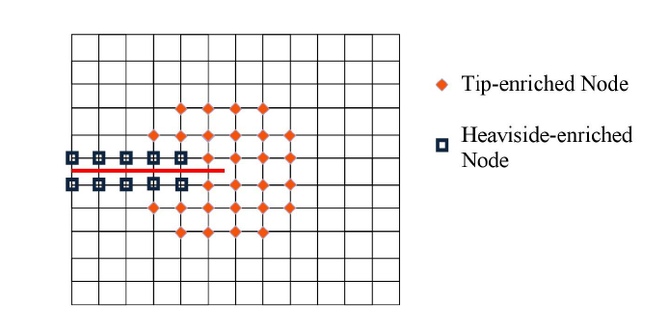
\includegraphics[scale=.3]{enrich.png}
     \caption{\hspace{-2cm}\footnotesize XFEM enrichment strategy}
  \end{figure}
\end{frame}
%%%%%%%%%%%%%%%%%%%%%%%%%%%%%%%%%%%%%%%%%%%%%%%%%%%%%%%%%%%%%%%%%%%%%%%%%%%%
%%%%%%%%%%%%%%%%%%%%%%%%%%%%%%%%%%%%%%%%%%%%%%%%%%%%%%%%%%%%%%%%%%%%%%%%%%%%
\begin{frame}[t,fragile]{\ldots Extended Finite Element Method}
    \vspace{-.3cm}
     \footnotesize
    \begin{itemize}
        \item The nodes which belongs to the elements totally cut by the crack, are enriched by and Heaviside function.
    $$h(x,y)=\begin{cases}1,&       for ~ ~ y\ge 0\\ -1,&       for~ ~ y\le 0\end{cases}$$
\item The nodes of elements which contains cracktip are enriched by $\gamma$:
     \footnotesize
    \begin{align*}
    u^h&=\sum_i N_i(x)u_i+\sum_{j\in J} N_j(x) h(x)a_j+\sum_{k\in K} N_k(x)\left( \sum_{l=1}^{4}\gamma_l(x)b_{kl} \right) \\
    v^h&=\sum_i N_i(x)v_i+\sum_{j\in J} N_j(x) h(x)c_j+\sum_{k\in K} N_k(x)\left( \sum_{l=1}^{4}\gamma_l(x)d_{kl} \right) \\ 
    where,\ \ \ \gamma&=\left[ \sqrt{r}\cos \left( \frac{\theta}{2} \right), \sqrt{r}\sin\left( \frac{\theta}{2} \right),\sqrt{r}\sin\left( \frac{\theta}{2} \right)\sin(\theta),\sqrt{r}\cos\left( \frac{\theta}{2} \right)\sin(\theta)\right] 
\end{align*}
\end{itemize}
\tiny
\hspace{10pt}
\textbf{Source:}Belytschko, T., \& Black, T. (1999). Elastic crack growth in finite elements with minimal remeshing. \\
\vspace{-7pt}
\hspace{10pt}
\emph{International journal for numerical methods in engineering}, 45(5), 601-620.
\end{frame}
%%%%%%%%%%%%%%%%%%%%%%%%%%%%%%%%%%%%%%%%%%%%%%%%%%%%%%%%%%%%%%%%%%%%%%%%
\begin{frame}[t,fragile]{Level Set Method}
    \vspace{-.3cm}
    \footnotesize
    \begin{itemize}
        \item The position of crack can be defined by level set methods. There are two level-set functions:
          \begin{itemize}
        \item Normal level set, $\psi(x)=$ the signed distance from the crack surface.
        \item Tangent level set, $\phi(x)=$ the signed distance to the plane including the crack front and perpendicular to the crack surface.
        \end{itemize}
    \item To decide which enrichment should be used. 
        \begin{itemize}
            \item If $\phi < 0 $ and $\psi_{min}\psi_{max}\leq 0$, nodes should be enriched with $h(x)$.
            \item If $\phi_{min}\phi_{max}\leq 0$ and $\psi_{min}\psi_{max}\leq 0 $, nodes should be enriched with $\gamma$.
        \end{itemize}
    \end{itemize}
  \begin{figure}
                \centering
                \vspace{-15pt}
                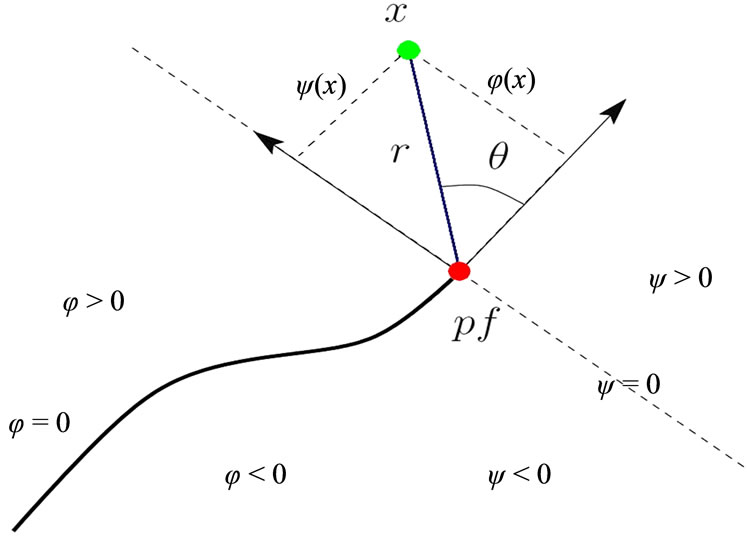
\includegraphics[scale=.15]{levelset.jpg}
                \caption{\tiny Level Set Method}
                \label{4}
            \end{figure}
    \tiny 
    \vspace{-20pt}
  \hspace{10pt}
    \textbf{Source:} Abdelaziz, Y., Bendahane, K., \& Baraka, A. (2011). Extended Finite Element Modeling: Basic Review and\\
  \vspace{-1pt}
  \hspace{10pt}
    Programming. Engineering, 3(07), 713.

\end{frame}
%%%%%%%%%%%%%%%%%%%%%%%%%%%%%%%%%%%%%%%%%%%%%%%%%%%%%%%%%%%%%%%%%%%%%%%%%%%%%%%
\begin{frame}[t,fragile]{Work done}
    \begin{itemize}
        \item Finite Element Formulation of coupled thermo-elastic problems
        \item MATLAB program is developed using the FEM formulation
        \item Patch test for the different modules of program is performed
        \item Various thermoelastic fracture problems are solved using the developed code 
        \item Need for using XFEM is shown by solving same problems and getting more accurate results 
    \end{itemize}
\end{frame}
%%%%%%%%%%%%%%%%%%%%%%%%%%%%%%%%%%%%%%%%%%%%%%%%%%%%%%%%%%%%%%%%%%%
\begin{frame}[t,fragile]{Finite Element Formulation of Thermo-elasticity}
\begin{itemize}
\item We will formulate the semi-coupled in which we neglect the effect of displacements on temperature field.
\item In thermoelastic case the total strain is given as: 
\begin{align}
    \varepsilon_{ij}&=\varepsilon_{ij}^{(M)}+\varepsilon_{ij}^{(T)}
    =\frac{1+\nu}{E}\sigma_{ij}-\frac{\nu}{E}\sigma_{kk}\delta_{ij}+\alpha(T-T_0)\delta_{ij}\nonumber
\end{align}
\item Which can be inverted to get following stress-strain relationship:
    \footnotesize
\begin{align*}
    \begin{Bmatrix}
        \sigma_{x}\\ \sigma_{y}\\ \tau_{xy} 
    \end{Bmatrix} =\frac{E}{(1-\nu^2)}
    \begin{bmatrix}
        1 & \nu & 0 \\ \nu & 1 & 0 \\ 0 & 0 & 1-\nu 
    \end{bmatrix}
    \begin{Bmatrix}
        \varepsilon_{x}-\alpha\Delta T \\ \varepsilon_{y}-\alpha \Delta T \\ \varepsilon_{xy} 
    \end{Bmatrix}
\end{align*}
\end{itemize}

\end{frame}
%%%%%%%%%%%%%%%%%%%%%%%%%%%%%%%%%%%%%%%%%%%%%%%%%%%%%%%%%%%%%%%
   \begin{frame}[t,fragile]{Finite element model}
    \begin{itemize}
        \item The governing equations of the thermo-elasticity is given by:
            \bgroup
            \tiny
            \begin{align*}
    \frac{\partial}{\partial x}\left[c_{11}\frac{\partial u}{\partial x}+c_{12}\frac{\partial v}{\partial y}\right]+&\frac{\partial}{\partial y}\left[c_{66}\left(\frac{\partial u}{\partial y}+\frac{\partial v}{\partial x}\right)\right]-(c_{11}+c_{12})\alpha\frac{\partial T}{\partial x}-f_x   =0 \\
    \frac{\partial}{\partial x}\left[c_{66}\left(\frac{\partial u}{\partial y}+\frac{\partial v}{\partial x}\right)\right]+&\frac{\partial}{\partial y}\left[c_{12}\frac{\partial u}{\partial x}+c_{22}\frac{\partial v}{\partial y}\right]-(c_{11}+c_{12})\alpha\frac{\partial T}{\partial y}-f_y=0\\
    &\ \ \ \ \ \ \ k\left( \frac{\partial^2 T}{\partial x^2}+\frac{\partial^2 T}{\partial y^2} \right)=q
\end{align*}
\egroup
where k is the thermal conductivity, T is temperature and q is the heat source.
      \item We can develop a week form of above equations by approximating u,v and T over a typical finite element $\Omega^e$ as:
          \footnotesize
\begin{align*}
    u(x,y)=\sum_{i=1}^nN_i (x,y)u_i\ \ , 
    v(x,y)=\sum_{i=1}^nN_i (x,y)v_i\ \ ,
    T(x,y)=\sum_{i=1}^nN_i (x,y)T_i
\end{align*}
\end{itemize}
\end{frame}
%%%%%%%%%%%%%%%%%%%%%%%%%%%%%%%%%%%%%%%%%%%%%%%%%%%%%%%%%%%%%%%%%%%%%%
\begin{frame}[t,fragile]{Weak form of Thermoelastic problem}
            \tiny
        \begin{align*}
     -\int_{\Omega}^{}\left[ c_{11}\frac{\partial N_i}{\partial x}\frac{\partial N_j}{\partial x}u_j+c_{12}\frac{\partial N_i}{\partial x}\frac{\partial N_j}{\partial y}v_j\right]dxdy+\int_{\Omega}^{}\left[c_{66}\frac{\partial N_i}{\partial y}\frac{\partial N_j}{\partial y}u_jdxdy+\frac{\partial N_i}{\partial y}\frac{\partial N_j}{\partial x}v_j\right]dxdy\nonumber\\ -\int_{\Omega}^{}\frac{\partial N_i}{\partial x}\beta N_jT_j dxdy +\int_{\Omega}^{}N_if_x
     dxdy+\int_{\Gamma}^{}N_i\vec{t}dx=0\end{align*}
 \begin{align*}
     -\int_{\Omega}^{}\left[ c_{11}\frac{\partial N_i}{\partial y}\frac{\partial N_j}{\partial y}v_j+c_{12}\frac{\partial N_i}{\partial y}\frac{\partial N_j}{\partial x}u_j\right]dxdy+\int_{\Omega}^{}\left[c_{66}\frac{\partial N_i}{\partial x}\frac{\partial N_j}{\partial x}v_jdxdy+\frac{\partial N_i}{\partial x}\frac{\partial N_j}{\partial y}u_j\right]dxdy\nonumber\\ -\int_{\Omega}^{}\frac{\partial N_i}{\partial y}\beta N_jT_j dxdy+\int_{\Omega}^{}N_if_y dxdy+\int_{\Gamma}^{}N_i\vec{t}dy=0\\
        k\int_{\Omega}\left( \frac{\partial N_i}{\partial x}\frac{\partial N_j}{\partial x}+\frac{\partial N_i}{\partial y}\frac{\partial N_j}{\partial y} \right)T_jdxdy-\int_{\Omega}^{}N_iN_jqdxdy=\int_{\Gamma}^{}N_i\bar{Q}ds& \end{align*}
\end{frame}
%%%%%%%%%%%%%%%%%%%%%%%%%%%%%%%%%%%%%%%%%%%%%%%%%%%%%%%%%%%%%%%%%%%
\begin{frame}[t,fragile]{weak form}
    Neglecting the body forces, above equations can be written in matrix form as follows\\ 
    \begin{align*}
\begin{bmatrix}
    K_{11} & K_{12} \\
    0 & K_{22}
\end{bmatrix}
\begin{Bmatrix}
    U^e\\ T^e
\end{Bmatrix}=
\begin{Bmatrix}
    F\\ Q
\end{Bmatrix}
\end{align*} 
 
    \tiny
    \begin{itemize}
        \item Where $U^e=[u~ ~ v]^T$ and $T^e$ are the unknown variables to be found and $K_{11}$, $K_{12}$ and $K_{22}$ are the stiffness matrices which are defined as below:\\  
\begin{align*}
K_{11}&=\int_{\Omega}^{}
\begin{bmatrix}
    c_{11}\frac{\partial N_i}{\partial x}\frac{\partial N_j}{\partial x}+c_{66}\frac{\partial N_i}{\partial y}\frac{\partial N_j}{\partial y} & c_{12}\frac{\partial N_i}{\partial x}\frac{\partial N_j}{\partial y}+c_{66}\frac{\partial N_i}{\partial y}\frac{\partial N_j}{\partial x}\\
    c_{12}\frac{\partial N_i}{\partial y}\frac{\partial N_j}{\partial x}+\frac{\partial N_i}{\partial x}\frac{\partial N_j}{\partial y}& c_{11}\frac{\partial N_i}{\partial y}\frac{\partial N_j}{\partial y}+c_{66}\frac{\partial N_i}{\partial x}\frac{\partial N_j}{\partial y}
\end{bmatrix}dxdy\\\\
K_{12}&=-\beta\int_{\Omega}^{}
\begin{bmatrix}
    \frac{\partial N_i}{\partial x}N_j \\ \frac{\partial N_i}{\partial y}N_j
\end{bmatrix}dxdy\\\\
K_{22}&=\int_{\Omega}^{}K\left( \frac{\partial N_i}{\partial x}\frac{\partial N_j}{\partial x}+\frac{\partial N_i}{\partial y}\frac{\partial N_j}{\partial y} \right)dxdy\\\\
F&= \int_{\Omega} N_i \begin{bmatrix} f_x\\f_y \end{bmatrix}dxdy~ ~ ~ ~ ~ ~ ~ ~ ~  ~ ~~ ~ ~ ~
Q=\int_{\Gamma}N_i\bar{Q}ds~ ~ ~ ~ and~ ~ ~ ~ U=[u~ ~ v]^T
\end{align*}
where the constants $c_{11}, c_{12}, c_{66}$
for plane strain is given by:
$$c_{11}=c_{22}=\frac{E(1-\nu)}{(1+\nu)(1-2\nu)}~ ~ ,~ ~ c_{12}=\frac{E\nu}{(1+\nu)(1-2\nu)}~ ~,~  ~ c_{66}=\frac{E}{1+\nu}$$
and for plane stress is given by: 
$$c_{11}=c_{22}=\frac{E}{(1-\nu^2)}~ ~ ,~ ~ c_{12}=\frac{E\nu}{(1-\nu^2)}~ ~,~  ~ c_{66}=\frac{E}{1+\nu}$$
\end{itemize}
\end{frame}
%%%%%%%%%%%%%%%%%%%%%%%%%%%%%%%%%%%%%%%%%%%%%%%%%%%%%%%%%%%%%%%%%%%%%%
\begin{frame}[t,fragile]{weak form}
    \tiny
         $$ N=\begin{bmatrix}N_1 &0&N_2 &0&\dots&N_n &0\\0&N_1 &0&N_2 &\dots&0&N_n \end{bmatrix}~and ~N^{\theta}=[N_1 ~\dots~N_n ] 
$$
Here $N$ and $N^{\theta}$ are the shape functions for displacement and temperature fields respectively. So the approximation of fields withing one element in matrix form can be written as:
$$ \begin{Bmatrix}u\\v\end{Bmatrix}=N\ U^e~ ~ ~ ~and ~ ~~ T=N^{\theta}\ T^e
$$
If we define the matrices $[B]$ and $[B^{\theta}]$ as follows:
    \begin{align}
    [B]=\begin{bmatrix}
        \frac{\partial N_1}{\partial x}&0&\frac{\partial N_2}{\partial x}&0&\dots&\frac{\partial N_n}{\partial x}&0\\
        0&\frac{\partial N_1}{\partial y}&0&\frac{\partial N_2}{\partial y}&\dots&0&\frac{\partial N_n}{\partial y}\\
\frac{\partial N_1}{\partial y}&\frac{\partial N_1}{\partial x}&
\frac{\partial N_2}{\partial y}&\frac{\partial N_2}{\partial x}&\dots&
\frac{\partial N_n}{\partial y}&\frac{\partial N_n}{\partial x}
    \end{bmatrix}~ ~ and ~ ~    [B^{\theta}]=\begin{bmatrix}
        \frac{\partial N_1}{\partial x}&\frac{\partial N_2}{\partial x}&\dots&\frac{\partial N_n}{\partial x}\\
        \frac{\partial N_1}{\partial y}&\frac{\partial N_2}{\partial y}&\dots&\frac{\partial N_n}{\partial y}\\
    \end{bmatrix}
    \end{align}
The strains $\{\varepsilon\}$ and temperature gradients $\{\theta'\}$ can be written as follows:
    \begin{align}
    \left\{ \varepsilon \right\}=\left[ B \right]\{ U^{(e)} \} ~ ,~ ~ ~ ~ ~ ~ ~ ~ ~  ~ \{\theta'\}=\left[ B^{\theta} \right]\{ T^{(e)} \} 
\end{align}   
\end{frame} 

%%%%%%%%%%%%%%%%%%%%%%%%%%%%%%%%%%%%%%%%%%%%%%%%%%%%%%%%%%%%%%%%%%%%%%%%%
\begin{frame}[t,fragile]{weak form}
    \tiny
\begin{itemize}
    \item These expressions can also be written in the matrix as described by Tian \cite{tian}:
\begin{align}
    [K_{11}^e]&=\int_{\Omega}[B]^T[C][B]dxdy\\
    [K_{12}^e]&=\int_{\Omega}[B]^T[\beta][N^{\theta}]dxdy\\
    [K_{22}^e]&=\int_{\Omega}[B^{\theta}]^T[K][B^{\theta}]dxdy
\end{align}
\begin{align}
    \{F\}&=\int_\Gamma [N]^T{\bar{t}}ds\\
    \{Q\}&=\int_\Gamma [N^{\theta}]^T\bar{Q}ds
\end{align}
\end{itemize}
\end{frame}
%%%%%%%%%%%%%%%%%%%%%%%%%%%%%%%%%%%%%%%%%%%%%%%%%%%%%%%%%%%%%%%%%%%%%%%%
\begin{frame}[t,fragile]{Computer implementation}
\begin{wrapfigure}{r}{0.5\textwidth}
  \begin{center}
      \vspace{-1.3cm}
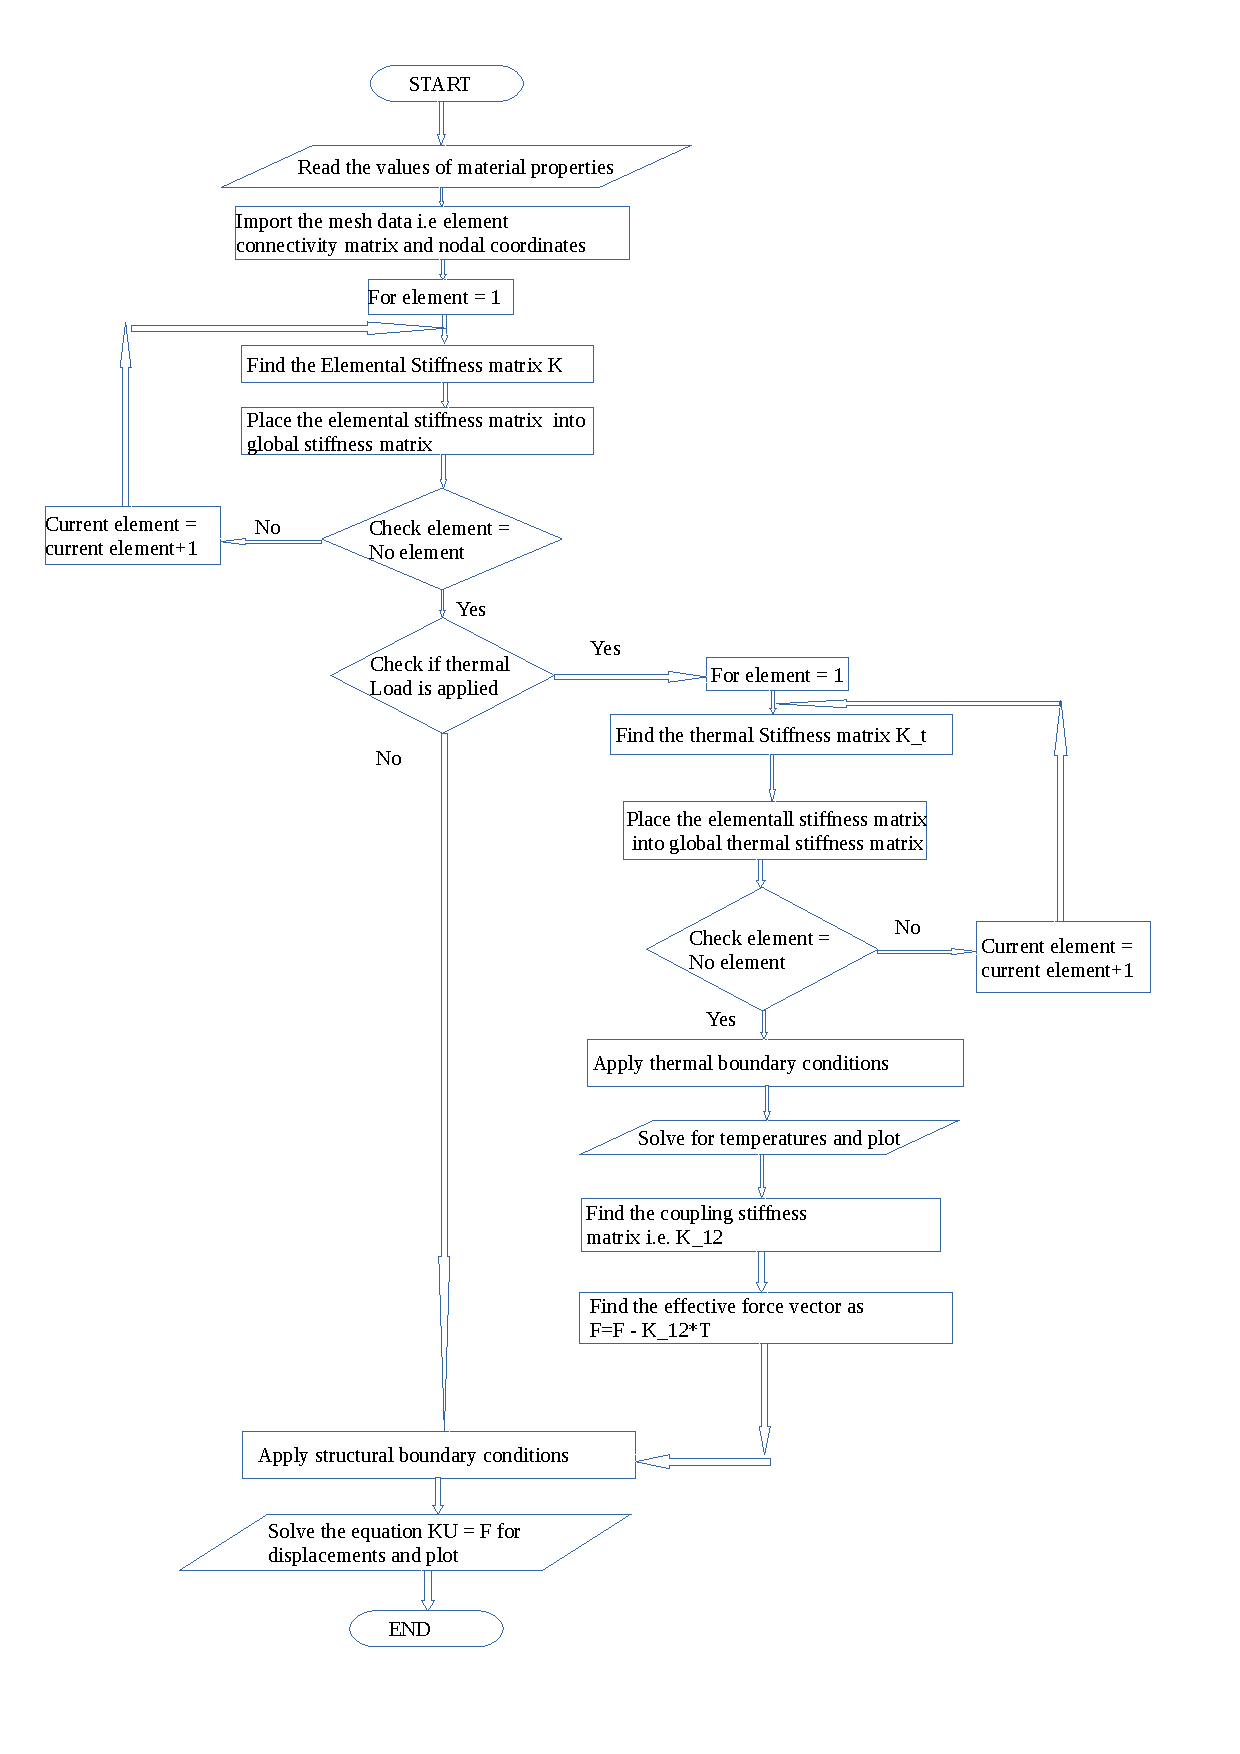
\includegraphics[width=0.48\textwidth]{flow_chart.pdf}
  \end{center}
\caption{Flowchart showing the steps of the FEM program}
\end{wrapfigure}
We have developed the 2-dimensional Finite Element Program and the elements used is quadrilateral elements i.e. Q4 elements. We transformed the quadrilateral element of a mesh to the master element $\hat{\Omega}$ (fig. and used $2\times 2$ Gauss quadrature rule for numerical integration.

\end{frame}
%%%%%%%%%%%%%%%%%%%%%%%%%%%%%%%%%%%%%%%%%%%%%%%%%%%%%%%%%%%%%%%%%%%%%
\begin{frame}[t,fragile]{Coupled Thermo-elasticity Problems}
    \begin{itemize}
        \item Coupled thermoelasticity problems have become very important in recent years because of its use in various industries.
        \item Some application areas include 
            \begin{itemize}
                \item aerodynamic heating of high speed air crafts as shown in figure (a). 
            \item the nuclear reactors where very high-temperatures and temperature gradients are developed as shown in figure (b).
            \item the ultra fast pulse lasers which is used for
micro-machining.
            \item non destructive detection.
            \item natural characterisation etc 
            \end{itemize}
    \end{itemize}
    \vspace{-.5cm}
    \begin{figure}[H]
      \hspace{.5cm}
\begin{subfigure}{0.45\textwidth}
  \vspace{.5cm}
    \centering
 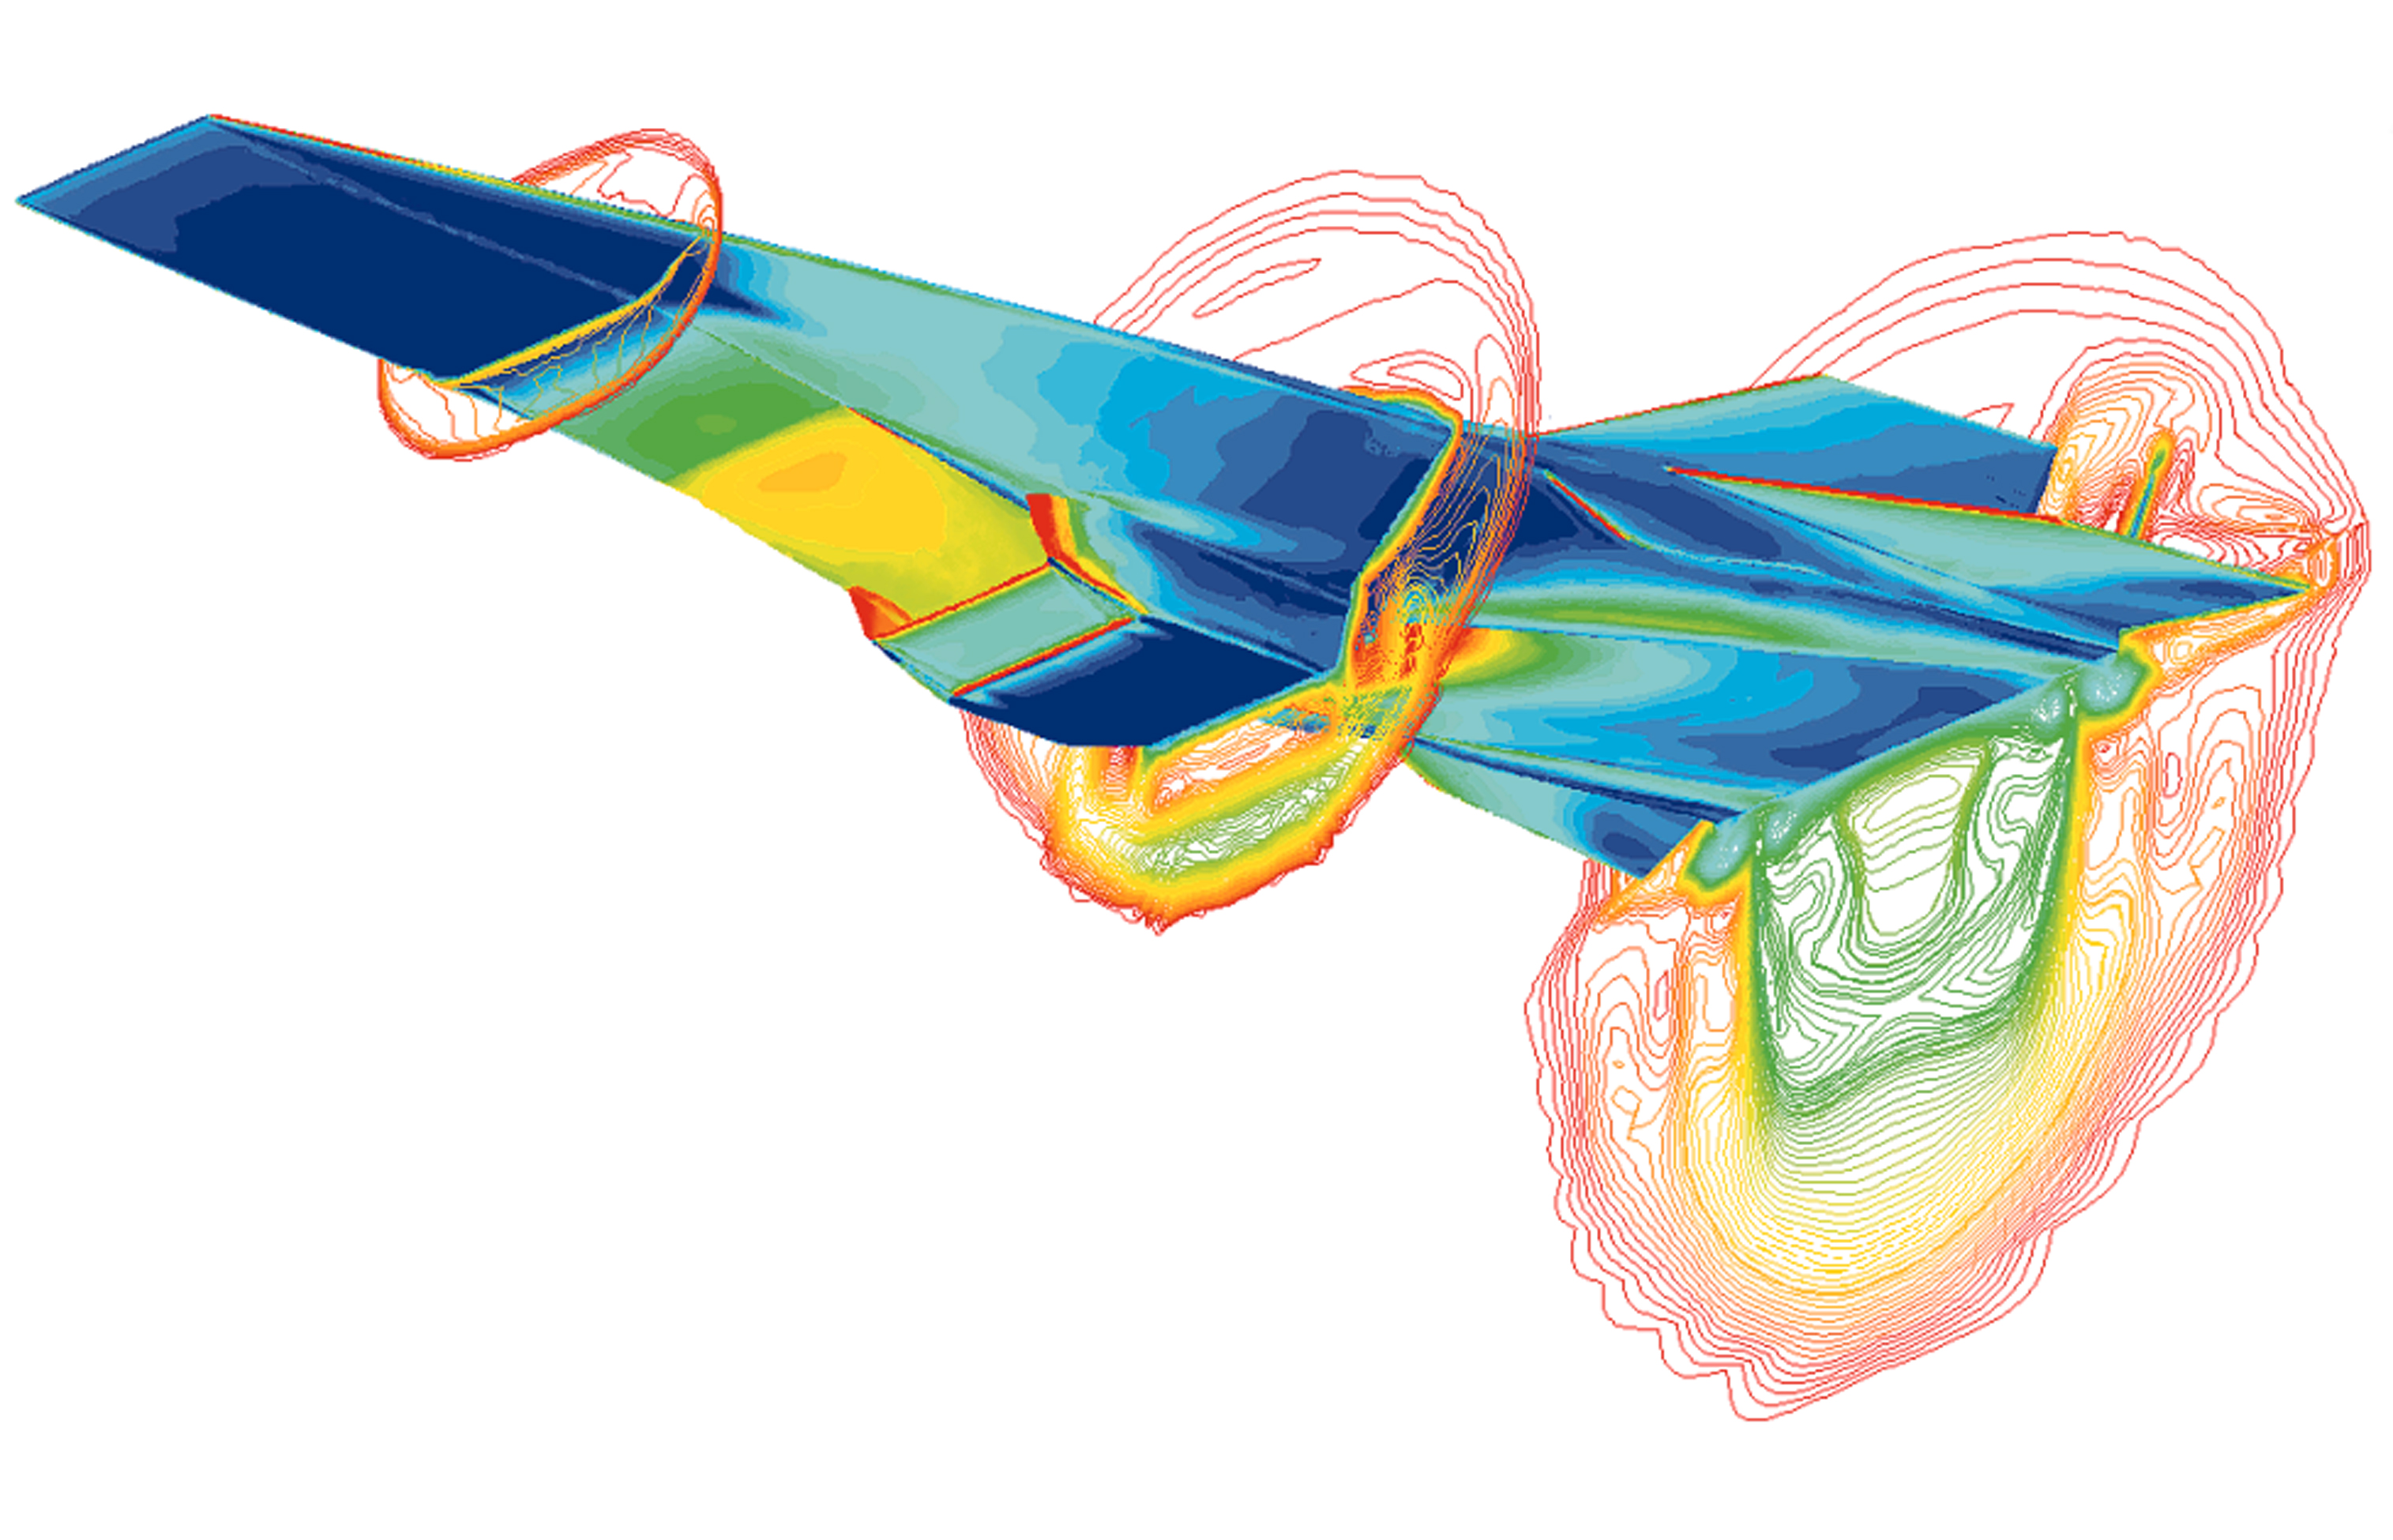
\includegraphics[scale=.1]{hyper.jpg}
 \caption{\tiny{Hyper-X vehicle at Mach 7.Source: www.dfrc.nasa.gov}}
 \end{subfigure}
 \begin{subfigure}{0.45\textwidth}
    \centering
 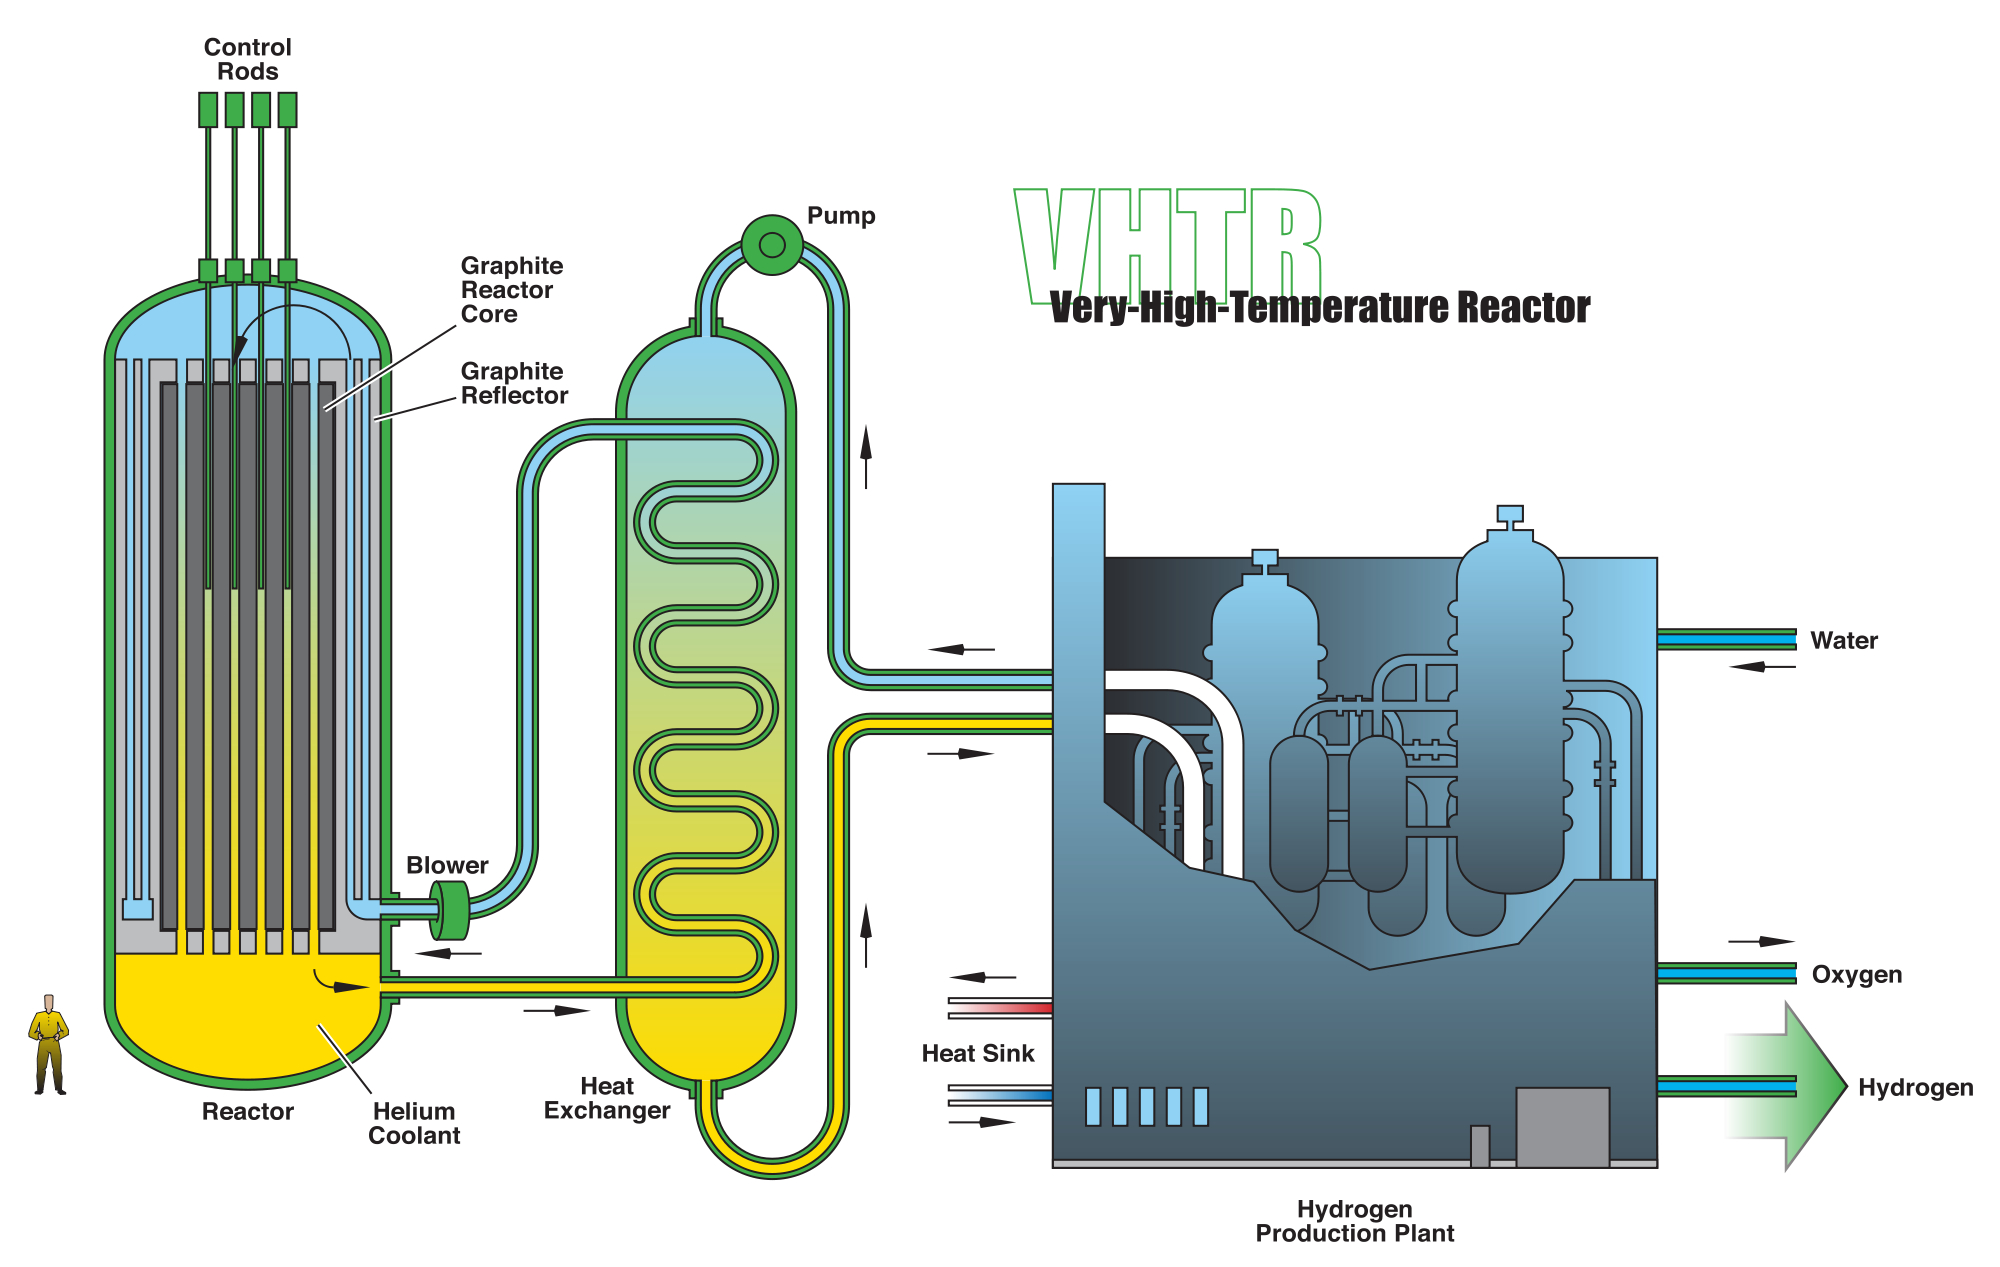
\includegraphics[scale=.05]{reator.png}
 \caption{\tiny{High temperature reactor. Source: https://commons.wikimedia.org}}
 \label{2}
 \end{subfigure}
\label{fig:caption}
\end{figure}
\end{frame}
%%%%%%%%%%%%%%%%%%%%%%%%%%%%%%%%%%%%%%%%%%%%%%%%%%%%%%%%%%%%%%%%%%%%%
%%%%%%%%%%%%%%%%%%%%%%%%%%%%%%%%%%%%%%%%%%%%%%%%%%%%%%%%%%%%%%%%%%%%%%%%%%%%
\end{document}


